\newpage
\section{Einleitung}
Digitale Bildverarbeitung wird unter anderem in industriellen Prozessen, medizinischen Verfahren oder in Multimedia-Produkten angewandt. In diesem Labor soll eine beispielhafte Multimedia-Anwendung entwickelt werden, die �ber das Labor hinaus als erheiterndes Demonstrationsobjekt f�r Bildverarbeitung in Videokonferenzen genutzt werden kann. Als Inspiration dient ein Effekt aus der Filmreihe \glqq Harry Potter\grqq .

\begin{figure}
	\centering
	\begin{minipage}{.45\textwidth}
		\centering
		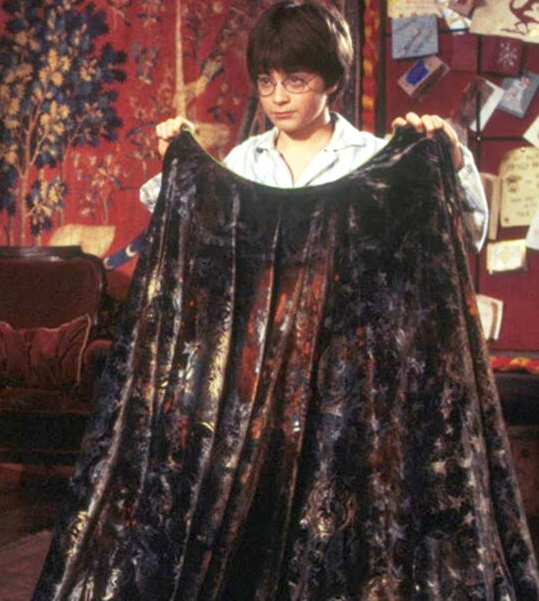
\includegraphics[width=.6\linewidth]{fig/harry1.jpg}
		\caption{Harry Potter ohne magischen Tarnumhang}
		\label{fig:harry1}
	\end{minipage}%
	\hspace{0.5cm}
	\begin{minipage}{.45\textwidth}
		\centering
		
\includegraphics[width=.6\linewidth]{fig/harry2.jpg}
		\caption{Harry Potter mit magischem Tarnumhang}
		\label{fig:harry2}
	\end{minipage}
\end{figure}

Die Abbildungen \ref{fig:harry1} und \ref{fig:harry2} zeigen Harry Potter ohne
\footnote{\url{https://assets.cdn.moviepilot.de/files/8a2cc0d2eb31c41136fb2be242540606dcd50821980e830481404b276065/fill/1280/614/Harry\%20Potter\%20Tarnumhang.jpg}} 
und mit\footnote{\url{https://www.tres-click.com/wp-content/uploads/2019/06/harry-potter-tarnumhang.gif}}
verzauberten Tarnumhang, welchen den Tr�ger des Umhangs verschwinden lassen kann. In diesem Labor entwickeln Sie eine Bildverarbeitungs-Pipeline, mit welcher dieser Effekt mit einer einfachen Webcam simuliert werden kann. Sie festigen den Umgang mit

\begin{itemize}
	\item Rauschunterdr�ckung
	\item Histogrammen 
	\item verschiedenen Farbr�umen
	\item Erosion und Dilatation
	\item Schwellwertverfahren 
\end{itemize}

und �ben gleichzeitig den Umgang mit der Programmiersprache Python.

\newpage
\subsection{Vorbereitung}
F�r das Labor wird ein Rechner mit Betriebssystem Windows, Linux-Ubuntu oder Mac ben�tigt. Zus�tzlich muss eine Webcam vorhanden sein (im Laptop integriert oder extern).
Melden Sie sich \textbf{vorab} bei dem Betreuer des Labors, sollte Ihnen eines der ben�tigten Mittel nicht zur  Verf�gung stehen.


Um an dem Labor erfolgreich teilnehmen zu k�nnen, muss die zu nutzende Programmierumgebung vorbereitet werden. Sollten Sie an der praktischen �bung zur Vorlesung \textit{Digitale Bildverarbeitung} teilgenommen haben, ist die erforderliche Programmierumgebung sowie der Programmcode wahrscheinlich bereits installiert und eingerichtet. Ansonsten befolgen Sie die Installationsanweisungen auf \url{https://github.com/TimoK93/Digitale-Bildverarbeitung} im Bereich \textit{0\_Einf�hrung}. Die Installation des Streaming Programms zur Erstellung einer virtuellen Kamera ist dabei optional und nicht verpflichtend.

Nachdem Sie die Installation vollendet haben, �ffnen Sie die Programmierumgebung, sodass Ihr Bildschirm �hnliches zu Abbildung \ref{fig:pycharm} anzeigt.

\begin{figure}
	\centering
	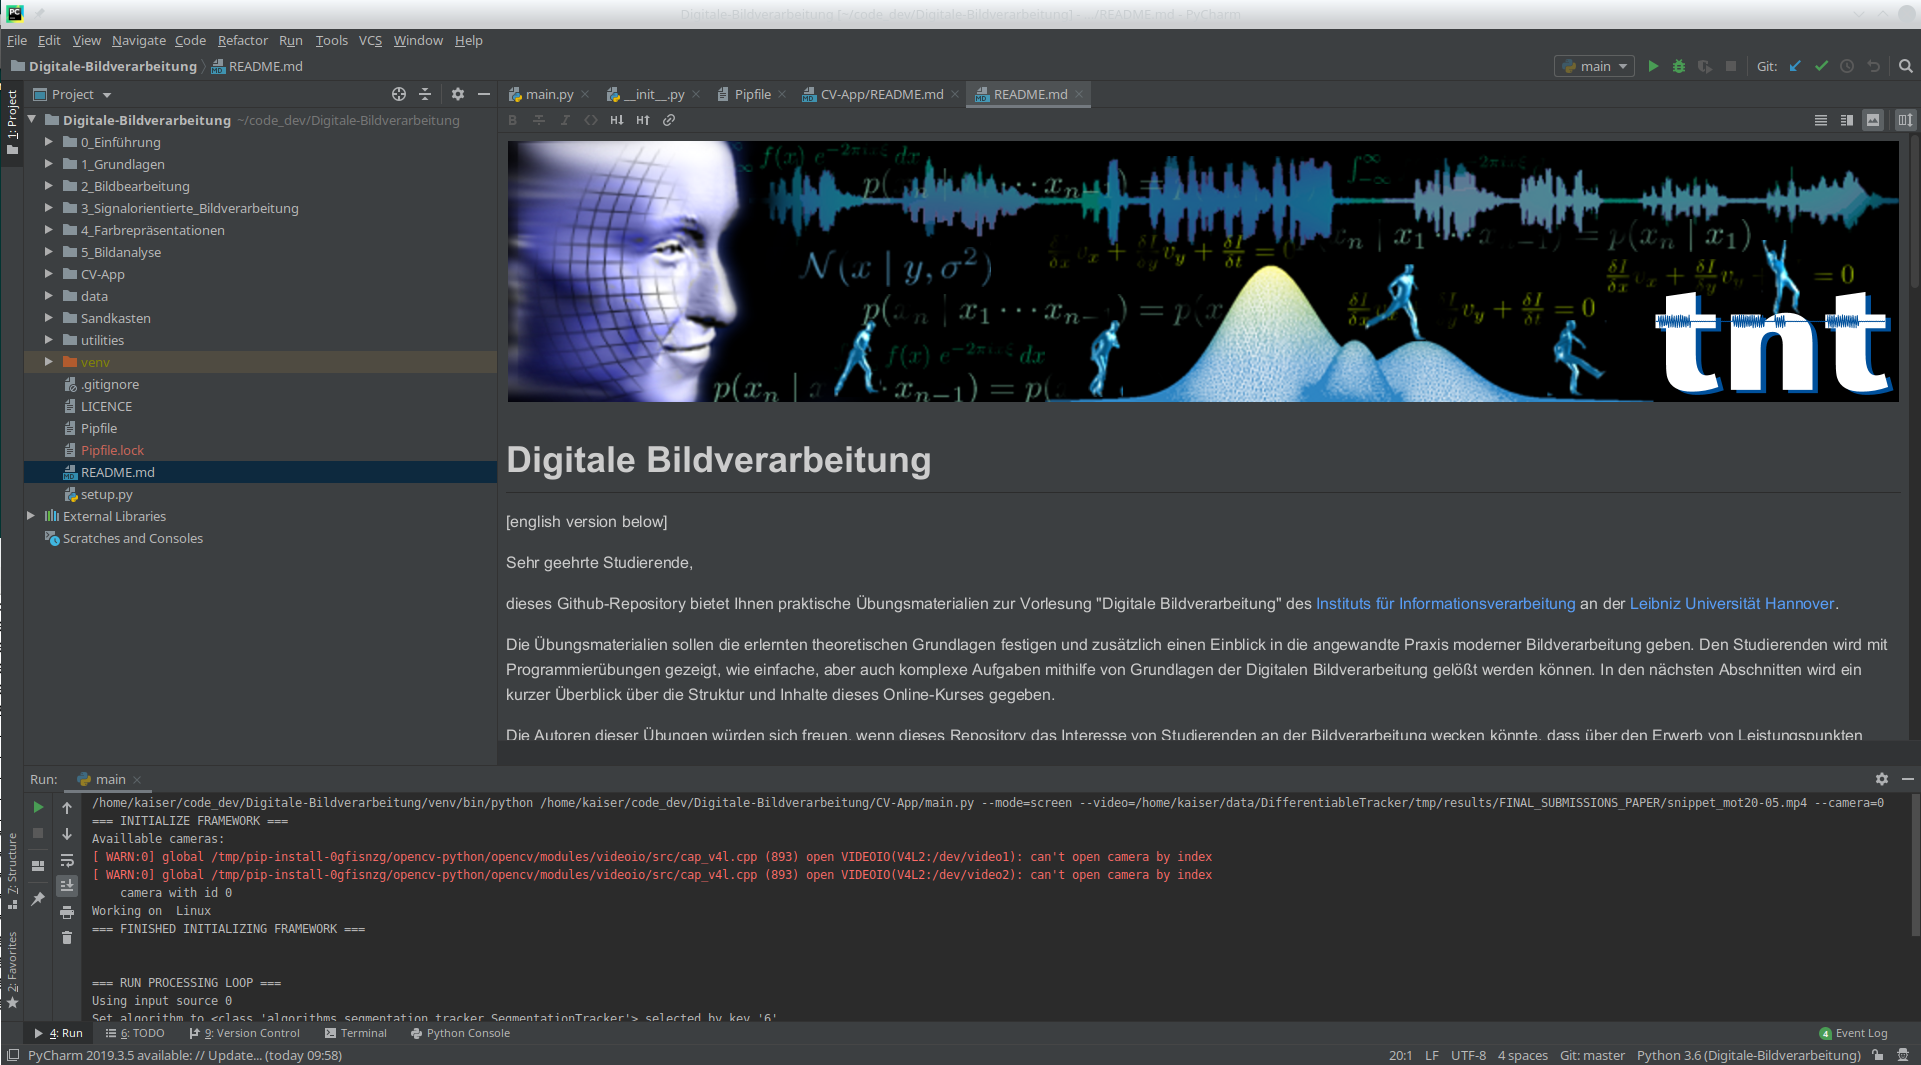
\includegraphics[width=\linewidth]{fig/pycharm.png}
	\caption{Programmierumgebung in PyCharm}
	\label{fig:pycharm}
\end{figure}

Machen Sie sich als n�chstes mithilfe der Beschreibung in Kapitel \ref{sec:Programmierumgebung} mit der Programmierumgebung vertraut. 



\newpage
\subsection{Programmierumgebung}  
\label{sec:Programmierumgebung}
In der Programmierumgebung ist das Hauptprogramm bereits soweit vorbereitet, sodass Sie einen Videostream aus Ihrer Kamera auslesen, darauf einen vorbereiteten Beispielalgorithmus anwenden und diesen anzeigen k�nnen. In diesem Kapitel wird kurz erl�utert, wie Sie diese Bildverarbeitungs-Pipeline starten und eigene Algorithmen integrieren k�nnen.

\paragraph*{Starten der Bildverarbeitungs-Pipeline.} �ffnen Sie die Datei \mbox{\textit{./CV-App/main.py}} in PyCharm und klicken Sie mit der rechten Maustaste in den Programmcode. �ffnen Sie dann das Fenster \textit{Modify Run Configuration...} wie in Abbildung \ref{fig:run_config} dargestellt. In dem Feld \textit{Parameter} k�nnen Sie zus�tzliche Argumente in die Umgebung eingeben. Argumente werden dabei im Schema \textit{--Argument1 Value1 --Argument2 Value2} eingegeben. Die einzustellenden Parameter k�nnen Sie aus der Tabelle \ref{tab:parameter} entnehmen. Wenn Sie keine Argumente w�hlen, werden die Standard Einstellungen gew�hlt.

\begin{table}
	\centering
	\caption{Argumente f�r die Programmausf�hrung}
	\begin{tabular}[h]{c | l| c}
		Argument & Werte & Default-Wert \\ \toprule
		 \textit{camera}	 & -1, 0, 1, \ldots (-1 �ffnet ein Video) & 0 \\
		 \textit{mode}	 & \textit{virtual\_cam} (virtuelle Kamera), \textit{screen} (nur Fenster)&  \textit{virtual\_cam} \\
		 \textit{video}	 & Pfad zu Video, wenn \textit{camera} den Wert $-1$ hat. & - \\
	\end{tabular}
		\label{tab:parameter}
\end{table}

\begin{figure}
	\centering
	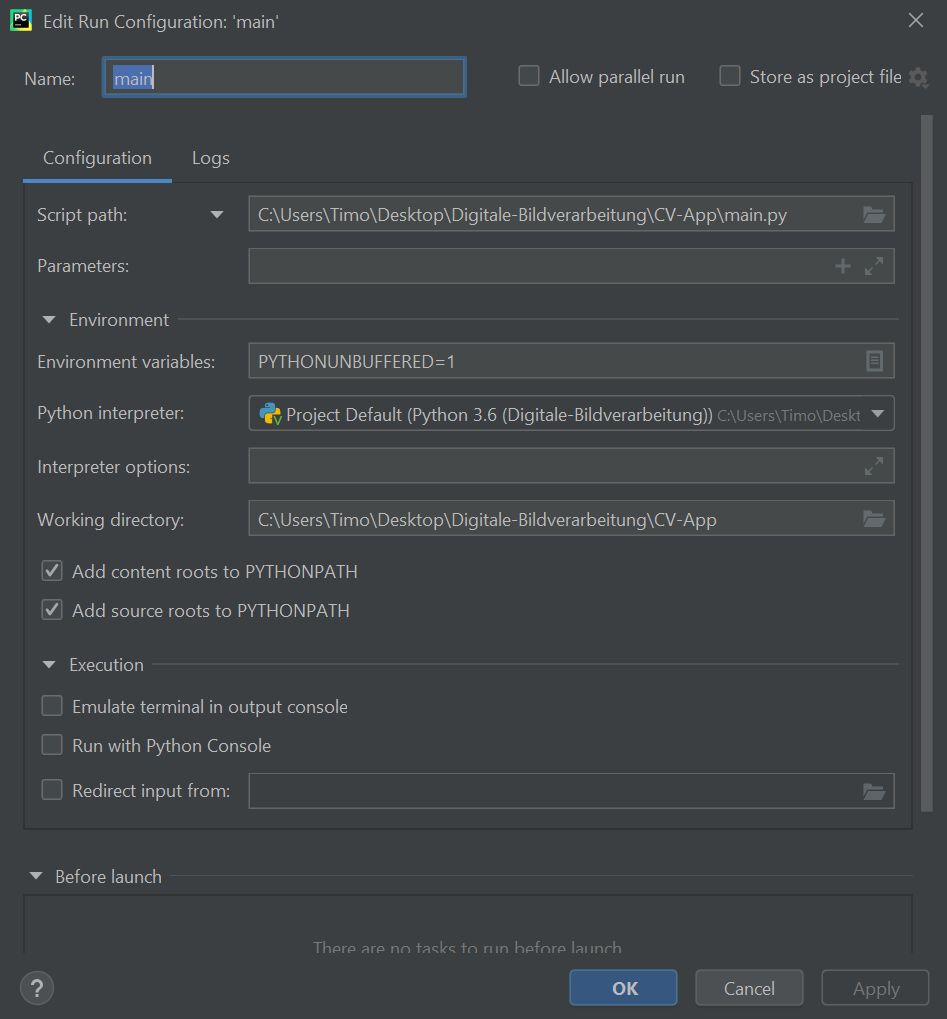
\includegraphics[width=0.65\linewidth]{fig/Run-Configs.png}
	\caption{Run Configuration in PyCharm}
	\label{fig:run_config}
\end{figure}

 Sie k�nnen das Programm nun mit \textit{Run} starten. Kurz nach dem Start sollten Sie ein Fenster mit dem Videostream aus Ihrer Kamera sehen. Durch das Bet�tigen verschiedener Tasten auf der Tastatur (z.B.\ Taste 1 oder 2) k�nnen Sie verschiedene Algorithmen aktivieren. Sie sehen das Ergebnis direkt in dem ausgegebenem Videostream. Wichtig: Das Programm reagiert nur auf Tastendr�cke, wenn das Videostream-Fenster im Vordergrund ihres Bildschirms ist.
 
 
 \paragraph*{Eigene Algorithmen einbinden.} F�r Sie sind nur die Dateien im Dateipfad \mbox{ \textit{./CV-App/algorithms}} relevant. Beispielhaft erstellen Sie im Folgenden den Algorithmus \textit{YourAlgorithm}.
 
 Erstellen Sie eine Datei \textit{your\_algorithm.py} und kopieren Sie den Inhalt aus dem Code \ref{lst:code2}. In der Funktion \textit{\_\_init\_\_(self)} k�nnen Sie dauerhafte Variablen definieren. Die Funktion \textit{process(self, img)} verarbeitet das Eingangsbild \textit{img} und gibt es am Ende modifiziert wieder aus (Hinweis: Ein und Ausgangsbild m�ssen gleich gro� sein!). Die Funktion \textit{mouse\_callback(self, ...)} reagiert auf Aktionen der Maus, wie zum Beispiel einem Mausklick an der Position x und y. So k�nnen Sie mit ihrem Algorithmus interagieren. Sie k�nnen sich einige Beispielalgorithmen in dem Ordner \textit{./CV-App/algorithms} zur Veranschaulichung ansehen. Der Algorithmus in \textit{white\_balancing.py} veranschaulicht alle Funktionen mit Algorithmen der Klasse \textit{Algorithm}.
 
  % Settings for listings
 \lstset{caption={Eigener Algorithmus in \textit{your\_algorithm.py}}}
 \lstset{label={lst:code2}}
 \begin{lstlisting}
import cv2
import numpy as np
from . import Algorithm

class YourAlgorithm(Algorithm):
    def __init__(self):
      self.some_persistent_value = "i_am_alwys_existing"
 
    def process(self, img):
        print(self.some_persistent_value)
        return img
 
    def mouse_callback(self, event, x, y, flags, param):
        if event == cv2.EVENT_LBUTTONUP:
            print("A Mouse click happend! at position", x, y)	 
 \end{lstlisting} 
 
 \newpage
 Um Ihren Algorithmus nun mit einer Aktivierungstaste-Taste zu verlinken, �ffnen Sie die Datei \textit{\_\_init\_\_.py}. Am Ende der Datei ist eine Verlinkung der Algorithmen zu bestimmten Tasten zu sehen (siehe Code \ref{lst:code1}).. In dem Beispiel in Code \ref{lst:code1} ist Ihr neuer Algorithmus \textit{YourAlgorithm} importiert und an die Taste 3 verlinkt. 
 
 % Settings for listings
 \lstset{caption={Verlinkung der Algorithmen in \textit{\_\_init\_\_.py}}}
 \lstset{label={lst:code1}}
 \begin{lstlisting}
from .image_to_gray import ImageToGray
from .image_to_hue import ImageToHue
from .your_algorithm import YourAlgorithm

algorithms = dict()
algorithms["0"] = Algorithm
algorithms["1"] = ImageToGray
algorithms["2"] = ImageToHue
algorithms["3"] = YourAlgorithm
 \end{lstlisting} 
 
 Nach Neustart des Programms durch erneute Bet�tigung der \textit{Run} Funktion, ist Ihr Algorithmus durch bet�tigen der Taste 3 zug�nglich.